\chapter{Grundlegendes}
\label{cha:grundlegendes}
% 3 Seiten

\section{Definition}

Deep Learning ist ein Gebiet aus dem maschinellen Lernen, das sich mit dem Trainieren von nicht linearen Modellen befasst, und hier meist mit vielschichtigen neuronalen Netzen befasst.\todo{mega geile referenz}

Deep Learning wird zum Beispiel zur Klassifizierung von Daten oder zur Extraktion von Merkmalen aus Daten eingesetzt.

\section{Entstehung}

Die Wurzeln des Deep Learnings gehen zurück in die 1950er Jahre, als Frank Rosenblatt eine Maschine namens Perceptron baute. Diese Maschine war in der Lage einige einfache Figuren wie Quadrate und Dreiecke zu erkennen. Für die damalige Zeit war das eine herausragende Maschine und regte den Gedanken, Maschinen zu bauen die Menschen imitieren können weiter an.

Knapp 20 Jahre später schrieb Marvin Minsky ein Buch das die Limitierungen der Maschine aufzeigte und einige scheinbar fundamentale Probleme aufwarf. Diese Erscheinung ließ die neuronalen Netze wieder in den Hintergrund rücken.
In den 1980er Jahren hat, der heute renomierte Wissenschaftler in diesem Bereich, eine Maschine gebaut die bereits eine versteckte Schicht besaß und somit in der Lage war komplexere Aufgaben zu lösen. In dieser Zeit entstand auch der erste Backpropagation Algorithmus\todo{ref Werbos, Amari?, Parker, LeCun, Rumelhart, ..)}. Das trainieren dieser Maschine war sehr aufwendig und so verschwand auch sie bald wieder von der Bildfläche. 

Erst mit einer Entdeckung 2006, erneut durch Geoff Hinton\todo{ref}, die den Backpropagation Algorithmus erheblich vereinfachte, haben neuronale Netze mit mehreren versteckten Schichten wieder an Bedeutung gewonnen. 

Heute stellen führende Unternehmen immer häufiger Teams rund um neuronale Netze und das Trainieren dieser zusammen um sich wirtschaftliche Vorteile zu sichern\todo{ref google, apple}. Erste Erfolge sieht man an Microsofts Spracherkennung Cortana\todo{ref}, Siri von Apple, Google Now oder der Bildersuche von Google, die mit Bildern ähnlichen Bildern sucht.


\section{Hürden}

Die aus der Vergangenheit bekannten Probleme beim Fortschritt neuronaler Netze mit vielen versteckten Schichten strecken sind zum größten Teil bis heute durch. Aktuelle Algorithmen aus dem Deep Learning tendieren zu Überanpassung, Unteranpassung, lokalen Minima oder kämpfen einfach mit der nicht vorhandenen Rechenleistung.

Grundsätzlich kann man für heute verwendete Algorithmen sagen, dass die Performance von neuronalen Netzen sehr stark von der Menge der Trainingsdaten und weniger von der Auswahl der Algorithmen abhängt. Nicht zuletzt hat die Verfügbarkeit von immensen Datenmengen von Unternehmen und aus dem Internet einen sehr positiven Einfluss auf das Interesse und die Entwicklungen im Bereich der Deep Learning Algorithmen.

%hidden layer nicht trainiert werden konnten (rechenpower außer bei time-delay und convolutional nets) + hat nicht für netzwerke mit feedback funktioniert

\section{Neuronale netze}

\begin{figure}
	\centering
	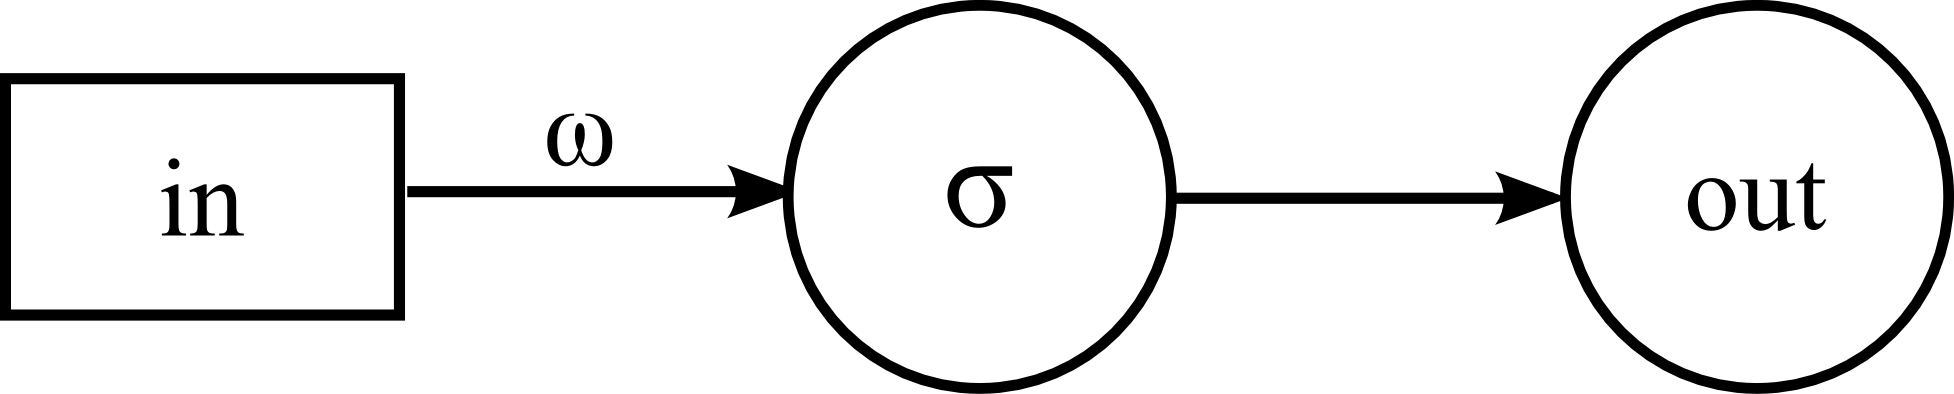
\includegraphics[scale=1]{images/neuron.png}
	\caption{Neuron}
	\label{fig:neuron}
\end{figure}

Neuronale Netze sind Strukturen aus der Technik, die dem Nervensystem von Lebewesen ähneln. Es sind Modelle, die Eingangsdaten über Neuronen gewichtet kombinieren und daraus einen Ausgang errechnen. Neuronale Netze sind in der Technik zur Vereinfachung meist in mehreren Schichten aufgebaut.

Abbildung \ref{fig:neuron} zeigt ein einfaches Neuron mit einem Eingang. Ein Eingang wird mit dem Gewicht multipliziert um dann anhand der Übertragungsfunktion den Ausgang zu berechnen. Als Übertragungsfunktion dient meist die Sigmoid-Funktion, welche sich einfach differenzieren lässt und sich daher besonders gut eignet. Der Ausgang $out$ dieses Neurons ergibt sich somit aus der dem Eingang $in$ multipliziert mit dem Gewicht $\omega$ in der Sigmoid-Funktion $\sigma$.
$$out = \sigma(\omega * in)$$

\begin{figure}
	\centering
	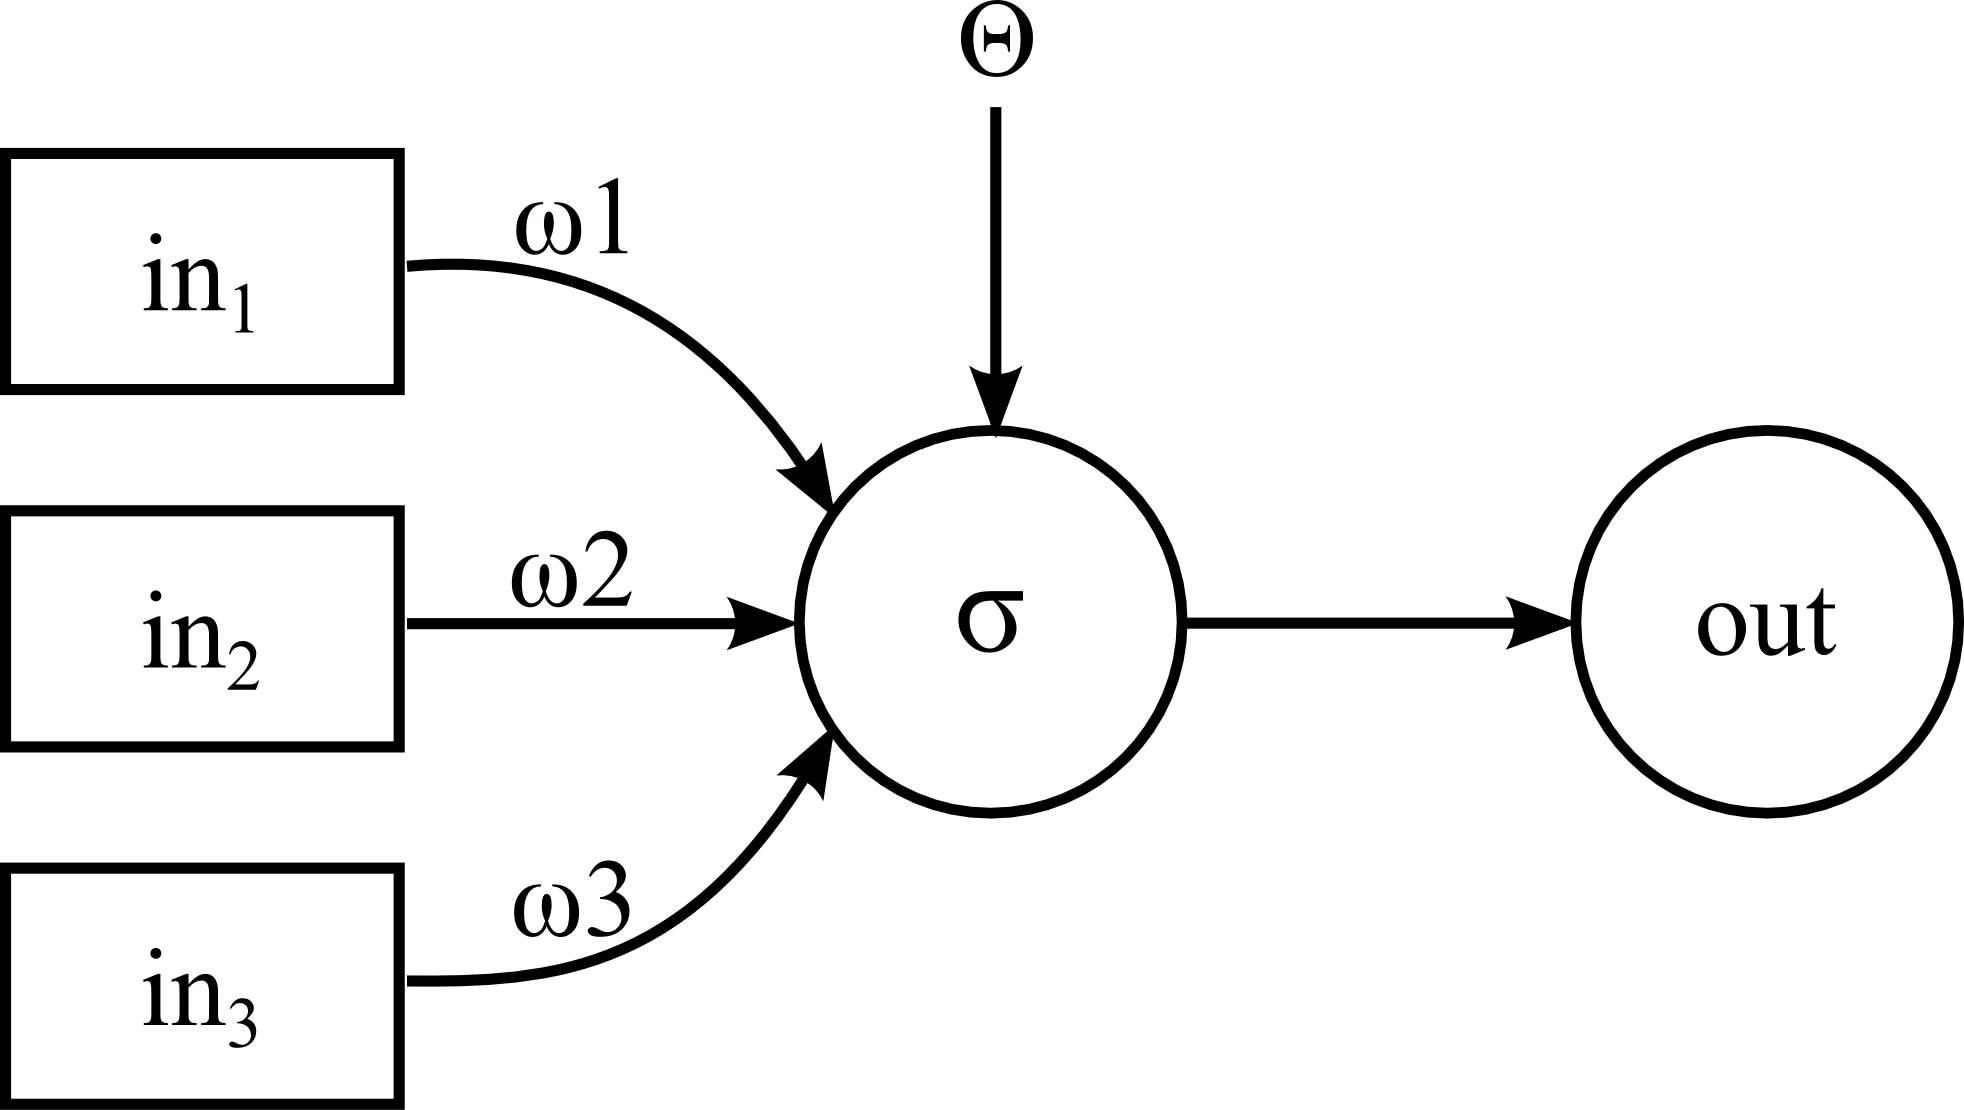
\includegraphics[scale=1]{images/neuron-multiple-inputs.png}
	\caption{Neuron mit mehreren Eingängen}
	\label{fig:neuron-multiple-inputs}
\end{figure}

Ein Neuron hat in der Regel, wie in Abbildung \ref{fig:neuron-multiple-inputs} zu sehen, mehrere Eingänge. Außerdem wird noch ein Bias-Wert $\theta$ für die Sigmoid-Funktion hinzugefügt. Der Ausgang dieses Neurons kann somit wie folgt berechnet werden:
$$out = \sigma(\omega_1*in_1 + \omega_2*in_2 + \omega_3*in_3 + \theta)$$

\begin{figure}
	\centering
	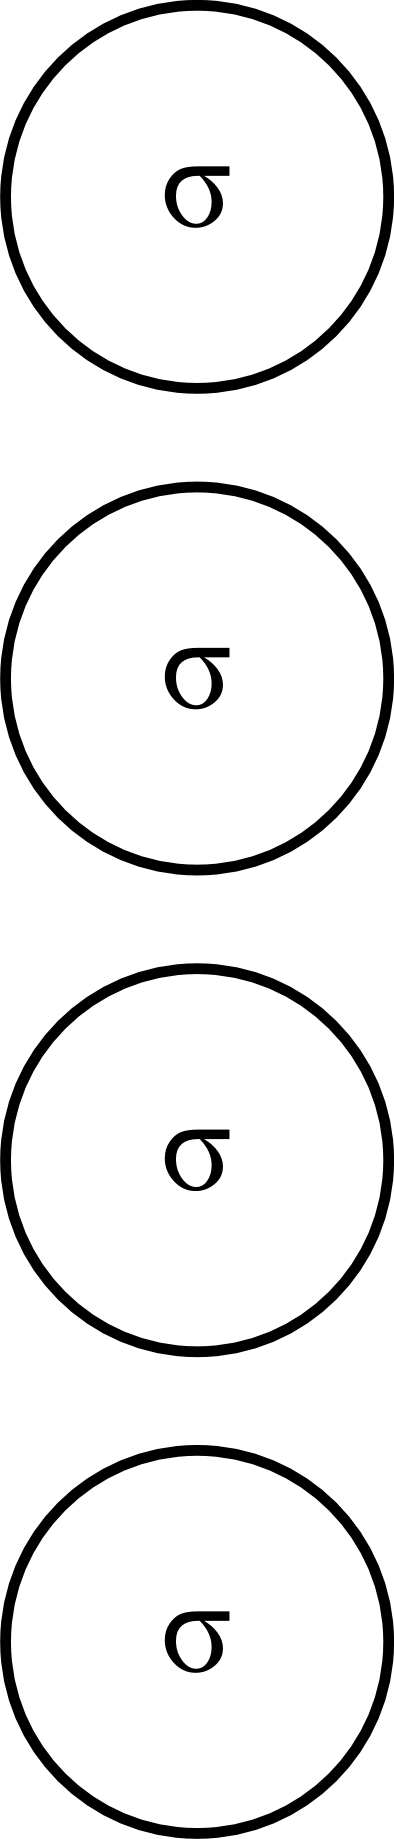
\includegraphics[scale=1]{images/neuron-layer.png}
	\caption{Layer von Neuronen}
	\label{fig:neuron-layer}
\end{figure}

\begin{figure}
\centering
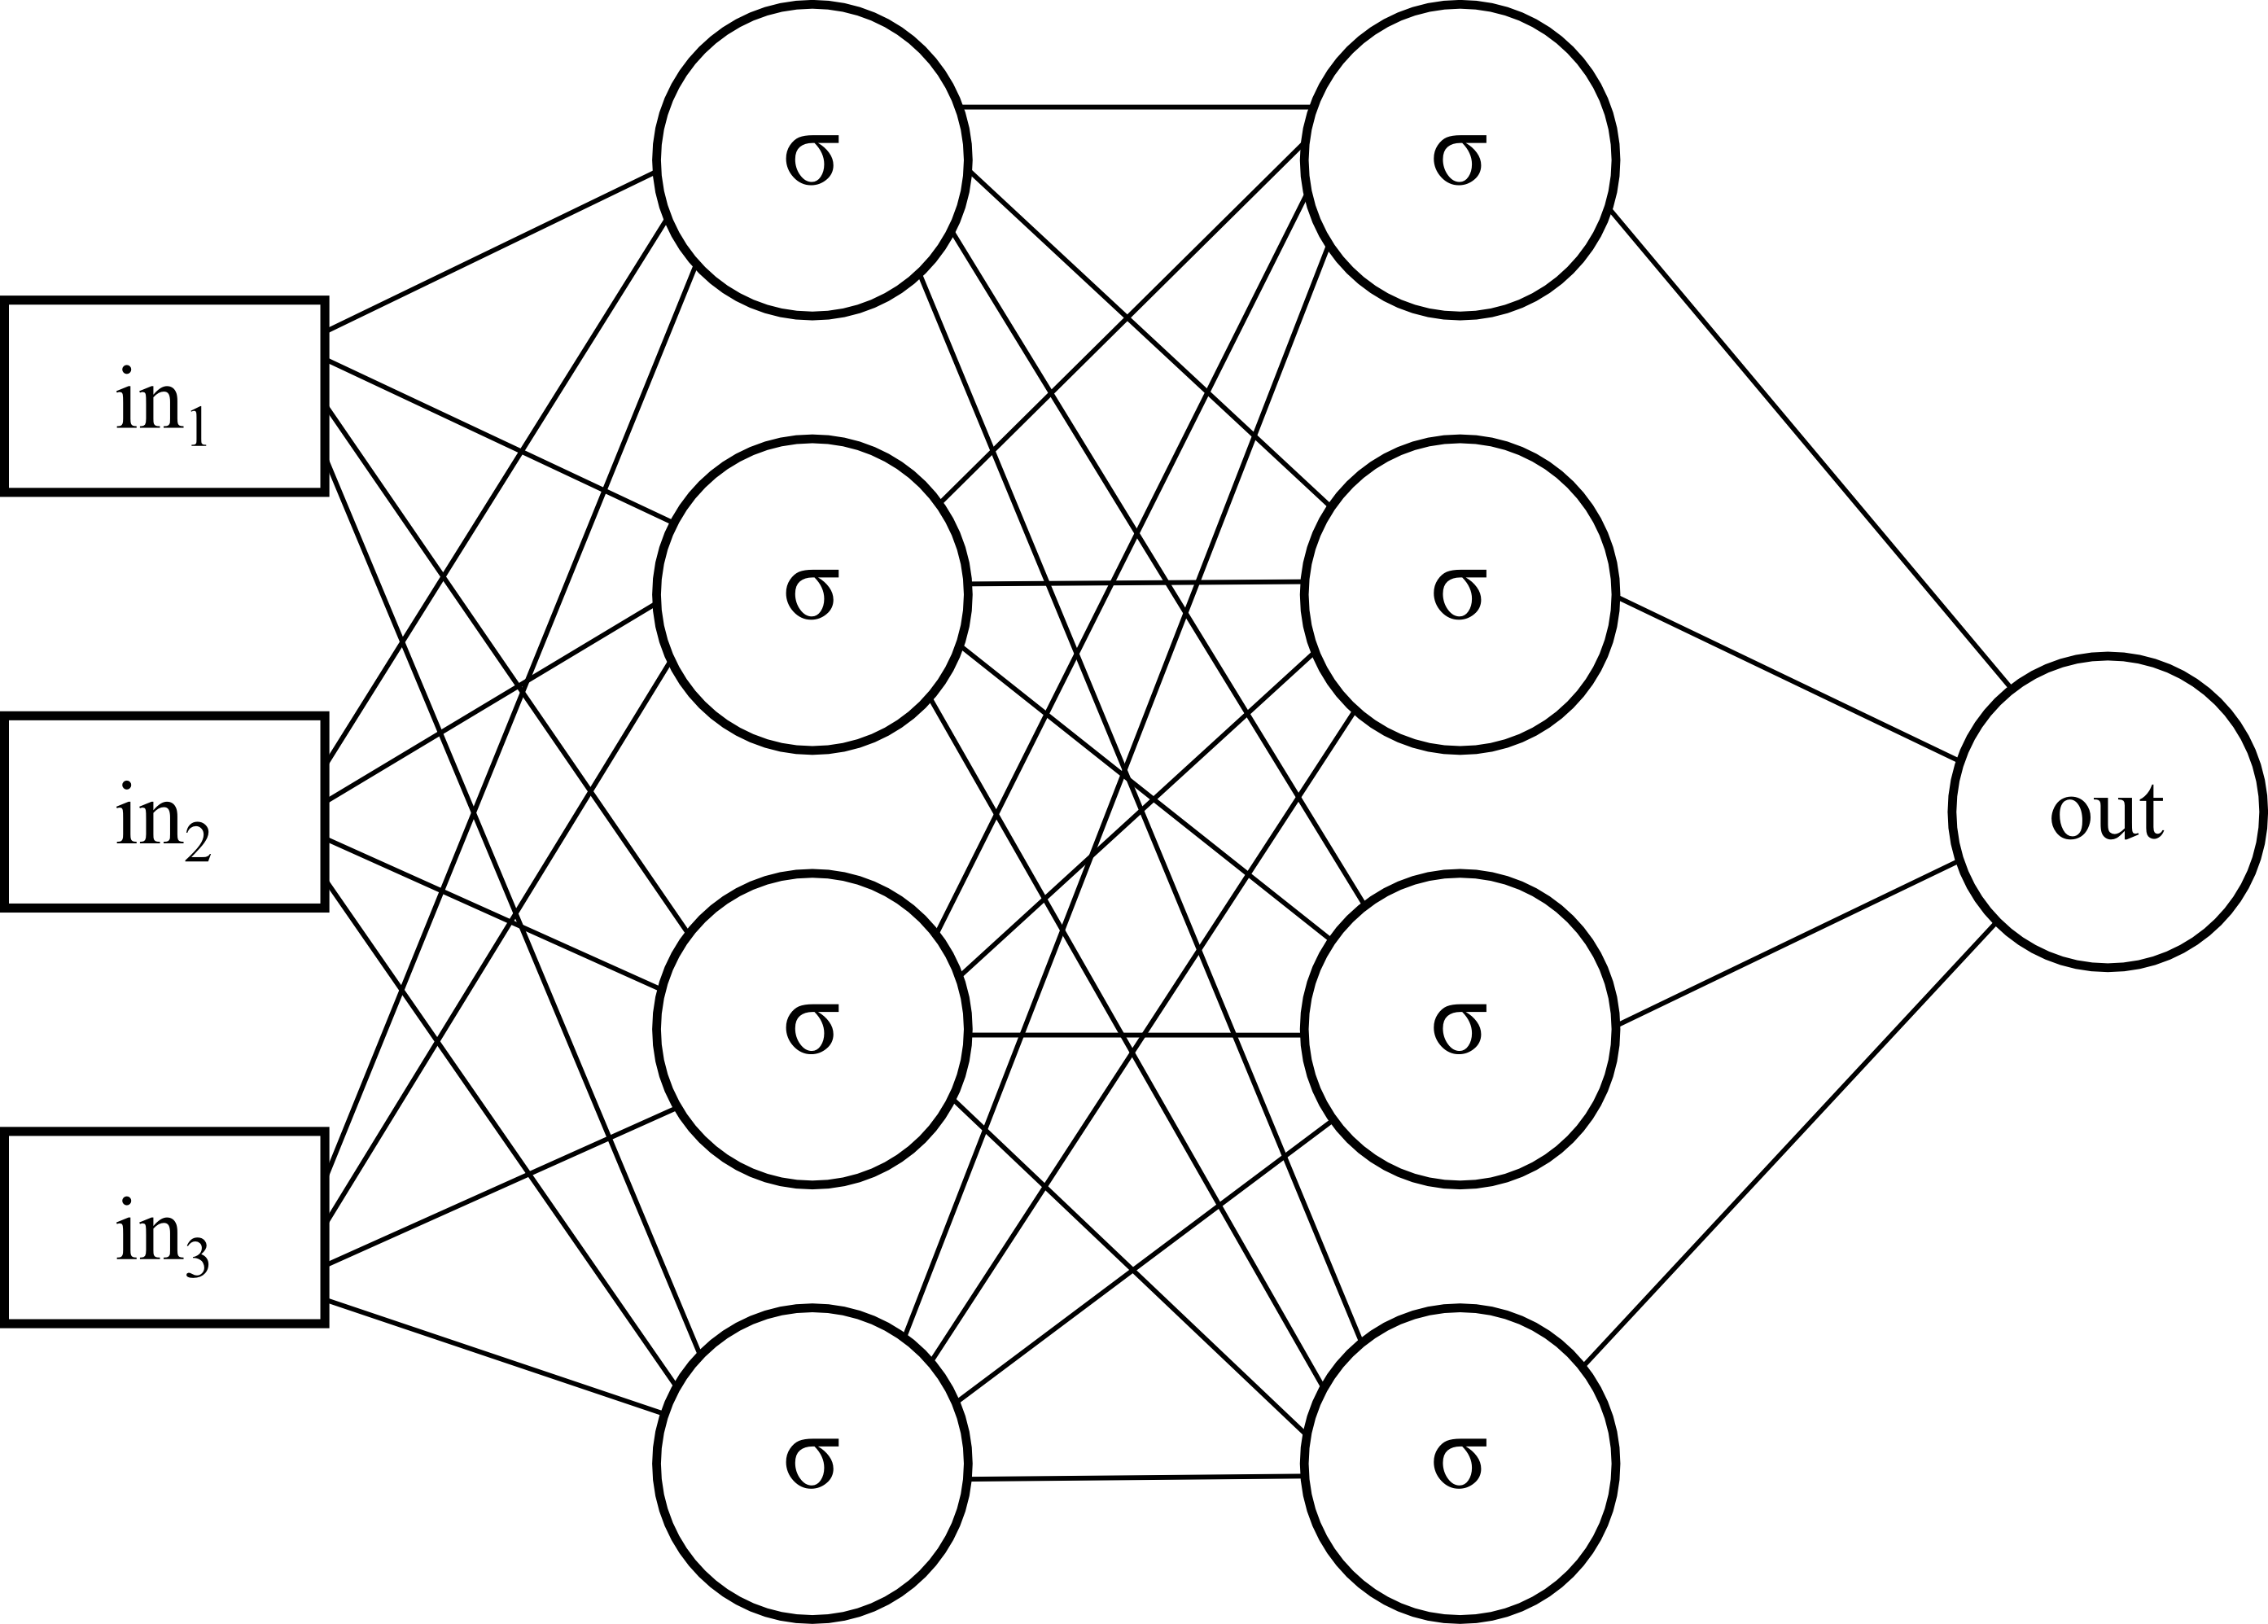
\includegraphics[scale=1]{images/neuron-network.png}
\caption{Ein Neuron}
\label{fig:neuron-network}
\end{figure}

Um aus den einzelnen Neuronen ein Netzwerk zu machen, werden, wie in Abbildung \ref{fig:neuron-layer} Layer gebildet. Ein Layer ist eine Menge an Neuronen, die untereinander nicht direkt verknüpft sind. Layer werden sequenziell hintereinander gehängt, wobei jedes Neuron eines Layers als Eingang für jedes Neuron des jeweils nächsten Layers dient. Ein solches Netzwerk ist auch in Abbildung \ref{fig:neuron-network} zu sehen. Dieses Netzwerk hat einen Layer für die Eingabedaten, einen für die Ausgabedaten und zwei innere Layer. Die inneren Layer werden als von außen Unsichtbar betrachtet und daher auch als Hidden-Layer bezeichnet.

\section{Überwacht / Unüberwacht}

Die Algorithmen des Deep Learning werden im groben in zwei Kategorien geteilt, in die überwachten und die unüberwachten Methoden. Überwacht bedeutet, dass Eingangsdaten an das System angelegt werden, für die die gewünschten Ausgangsdaten bekannt sind. Das könnte zum Beispiel heißen, dass das Netz Bilder mit und ohne Gesichtern darauf bekommt und dann anhand der Richtigkeit des Ausgangs das Modell angepasst wird.

Diese Art des Lernens scheint logisch, benötigt aber sehr viele Kategorisierte Datensätze, die nicht immer verfügbar sind und tendiert leicht zur Überanpassung. Überanpassung bedeutet, dass das Netz die Trainingsdaten besser als notwendig lernt und für weitere Eingabedaten schlechtere Ergebnisse liefert als wäre es weniger trainiert worden.

Ein weitere Ansatz ist das unüberwachte Lernen, es handelt sich dabei um Algorithmen, die lediglich Eingangsdaten benötigen. Die Grundlegende Idee dabei ist es, das Netz Merkmale aus den Eingangsdaten erkennen zu lassen. Unüberwachtes Lernen ist besonders wegen der enormen Verfügbarkeit unkategorisierten Daten interessant und wird häufig als Grundlage vor dem überwachten Lernen eingesetzt. Es hilft einige Probleme des überwachten Lernens zu verbessern, so können die Gewichte aus dem unüberwachten Lernen als Startwert für ein überwachtes Lernen eingesetzt werden. Diese Gewichte haben mehr Aussagekraft über Merkmale der Eingangsdaten als zufällige Werte und können mit weniger kategorisierten Trainingsdaten oft bessere Ergebnisse erzielt werden.